\documentclass[11pt,a4paper]{article}

% ---------------------------------------------------------------------------
% Paketi
% ---------------------------------------------------------------------------
\usepackage[utf8]{inputenc}
\usepackage[T1]{fontenc}
\usepackage[serbian]{babel}
\usepackage{amsmath,amssymb}
\usepackage{graphicx}
\usepackage{booktabs}
\usepackage{caption}
\usepackage{subcaption}
\usepackage{hyperref}
\usepackage{geometry}
\usepackage{xcolor}
\usepackage{listings}
\geometry{margin=2.5cm}

\hypersetup{
  colorlinks=true,
  linkcolor=blue!50!black,
  citecolor=green!50!black,
  urlcolor=blue!60!black
}

% Stil za prikaz koda
\lstset{
  basicstyle=\ttfamily\footnotesize,
  breaklines=true,
  frame=single,
  numbers=left,
  numberstyle=\tiny\color{gray},
  keywordstyle=\color{blue!60!black},
  commentstyle=\color{green!50!black},
  stringstyle=\color{red!60!black},
  showstringspaces=false,
  language=Python
}

% ---------------------------------------------------------------------------
% Naslov
% ---------------------------------------------------------------------------
\title{\textbf{Detekcija vozila na slikama pomo\'cu\\konvolucionih neuronskih mre\v za}}
\author{%
  Aleksa Vukadinovi\'c\\
  \small Fakultet / Katedra\\
  \small Predmet: Ra\v cunarska inteligencija
}
\date{\today}

\begin{document}

\maketitle

\begin{abstract}
\noindent
U ovom radu razmatramo problem \emph{detekcije vozila} kao zadatak binarne
klasifikacije slika: odlu\v civanje da li data slika sadr\v zi vozilo.
Reprodukujemo dobro utemeljenu paradigmu konvolucionih neuronskih mre\v za
(KNM) koju su uveli LeCun i saradnici~\cite{lecun1998gradient} i Krizhevsky i
saradnici~\cite{krizhevsky2012imagenet}, implementiraju\'ci kompaktnu mre\v zu
u stilu VGG~\cite{simonyan2015very} sa normalizacijom po grupama (engl.
\emph{batch normalization})~\cite{ioffe2015batch} i regularizacijom odbacivanjem
(engl. \emph{dropout})~\cite{srivastava2014dropout}. Model je treniran i
evaluiran na skupu podataka CIFAR-10~\cite{krizhevsky2009learning}, \v cijih
deset klasa preslikavamo u binarne ciljeve \emph{vozilo} i \emph{nije vozilo}.
Da bismo kvantifikovali doprinos konvolucione arhitekture, upore\dj ujemo KNM
sa dva jednostavnija, samostalno razvijena referentna metoda (logisti\v cka
regresija i potpuno povezana vi\v seslojna perceptronska mre\v za) trenirana na
sirovim pikselima. KNM posti\v ze ta\v cnost od $97.27\%$ na test skupu i
ROC-AUC od $0.9965$, \v cime zna\v cajno nadma\v suje referentne metode --
logisti\v cku regresiju ($81.56\%$) i MLP ($88.04\%$) -- \v sto potvr\dj uje
vrednost prostornog izdvajanja obele\v zja za ovaj zadatak.
\end{abstract}

\tableofcontents
\newpage

% ===========================================================================
\section{Uvod i pregled literature}
% ===========================================================================

\subsection{Opis problema}
Detekcija vozila je su\v stinski problem ra\v cunarskog vida sa primenama u
autonomnoj vo\v znji, nadzoru saobra\'caja i inteligentnim transportnim
sistemima. U svom naj\-op\-\v stijem obliku zahteva lokalizaciju svakog vozila
na slici pomo\'cu grani\v cnog okvira (engl. \emph{bounding box}). U ovom
projektu re\v savamo osnovni podproblem -- \emph{klasifikaciju prisustva
vozila}: za zadatu sliku fiksne veli\v cine treba odlu\v citi da li ona
prikazuje vozilo. Formalno, za sliku
$x \in \mathbb{R}^{3\times 32 \times 32}$ u\v cimo funkciju
$f_\theta : \mathbb{R}^{3\times 32 \times 32} \to \{0, 1\}$, gde $1$ ozna\v cava
,,vozilo'' a $0$ ,,nije vozilo''. Ovo je diskriminativni gradivni blok na kome
se grade detektori zasnovani na kliznom prozoru ili predlozima
regiona~\cite{ren2015faster,redmon2016you}.

\subsection{Nau\v cna pozadina i srodni radovi}
Upotreba konvolucionih neuronskih mre\v za za prepoznavanje slika datira jo\v s
od seminalne arhitekture LeNet koju su predlo\v zili LeCun i
saradnici~\cite{lecun1998gradient}, a koja je uvela obu\v cive konvolucione i
slojeve poduzorkovanja za prepoznavanje rukom pisanih cifara. Savremeni procvat
KNM zapo\v ceo je sa mre\v zom AlexNet~\cite{krizhevsky2012imagenet}, koja je
ubedljivo pobedila na takmi\v cenju ImageNet i pokazala da duboke KNM trenirane
na grafi\v ckim procesorima uz ReLU nelinearnosti dramati\v cno nadma\v suju
klasi\v cne tokove ra\v cunarskog vida zasnovane na ru\v cno konstruisanim
obele\v zjima poput histograma orijentisanih gradijenata
\cite{dalal2005histograms}. Naredni radovi produbili su i regularizovali ove
mre\v ze: VGG~\cite{simonyan2015very} je pokazao da slaganje malih $3\times 3$
konvolucija daje sna\v zne reprezentacije, dok je ResNet~\cite{he2016deep} uveo
rezidualne veze koje omogu\'cavaju veoma duboke modele. Dve tehnike
regularizacije i optimizacije danas su standardne i kori\v s\'cene su u ovom
radu: normalizacija po grupama~\cite{ioffe2015batch}, koja stabilizuje i
ubrzava treniranje, i odbacivanje~\cite{srivastava2014dropout}, koje smanjuje
preprilago\dj avanje. Za optimizaciju koristimo Adam~\cite{kingma2015adam} sa
razdvojenim opadanjem te\v zina~\cite{loshchilov2019decoupled} i kosinusnim
raspore\dj iva\v cem stope u\v cenja~\cite{loshchilov2017sgdr}. \v Sirok pregled
ovih ideja dat je u preglednom radu LeCun-a, Bengio-a i
Hinton-a~\cite{lecun2015deep} kao i u ud\v zbeniku Goodfellow-a i
saradnika~\cite{goodfellow2016deep}.

Za detekciju vozila na celoj slici (sa lokalizacijom), savremeni sistemi poput
Faster R-CNN~\cite{ren2015faster} i YOLO~\cite{redmon2016you} pro\v siruju
klasifikacionu KNM osnovu (engl. \emph{backbone}) glavama za predloge regiona
ili regresiju po mre\v zi. Na\v s klasifikator odgovara takvoj osnovi
ograni\v cenoj na binarnu odluku vozilo/nije-vozilo i mogao bi se, u principu,
ugraditi u detektor sa kliznim prozorom.

\subsection{Doprinos ovog rada}
Ovaj projekat je \emph{reprodukcija} utemeljene metodologije klasifikacije
slika pomo\'cu KNM primenjene na detekciju vozila; ne tvrdimo da je arhitektura
nova. Na\v si konkretni doprinosi su: (i) \v cista, reproducibilna implementacija
mre\v ze u stilu VGG u okviru PyTorch-a~\cite{paszke2019pytorch} za binarnu
klasifikaciju vozila; (ii) dve samostalno razvijene referentne metode
implementirane pomo\'cu biblioteke scikit-learn~\cite{pedregosa2011scikit} koje
izoluju efekat konvolucija; i (iii) temeljno eksperimentalno pore\dj enje sa
standardnim merama, krivama i kvalitativnim vizuelizacijama na jednostavnim
test primerima.

% ===========================================================================
\section{Opis na\v seg re\v senja}
% ===========================================================================

\subsection{Skup podataka i preslikavanje oznaka}
Koristimo skup podataka CIFAR-10~\cite{krizhevsky2009learning}, koji sadr\v zi
$60{,}000$ slika u boji veli\v cine $32\times 32$ piksela ravnomerno
raspore\dj enih u deset klasa ($50{,}000$ za treniranje, $10{,}000$ za
testiranje). Deset originalnih klasa preslikavamo u binarni cilj kao \v sto je
prikazano u Tabeli~\ref{tab:mapping}. \v Cetiri klase vezane za transport
postaju pozitivna klasa (vozilo), a \v sest klasa \v zivotinja postaje negativna
klasa (nije vozilo), \v sto daje odnos pozitivnih i negativnih primera od
$40\%/60\%$.

\begin{table}[h]
\centering
\caption{Preslikavanje klasa skupa CIFAR-10 u binarni cilj detekcije vozila.}
\label{tab:mapping}
\begin{tabular}{ll}
\toprule
\textbf{Cilj} & \textbf{Originalne klase CIFAR-10} \\
\midrule
$1$ -- vozilo      & avion, automobil, brod, kamion \\
$0$ -- nije vozilo & ptica, ma\v cka, jelen, pas, \v zaba, konj \\
\bottomrule
\end{tabular}
\end{table}

Zvani\v cni trening skup od $50{,}000$ slika dodatno se deli u odnosu
$90\%/10\%$ na trening i validacioni podskup. Validacioni podskup koristi se za
izbor modela (\v cuvamo kontrolnu ta\v cku sa najve\'com validacionom
ta\v cno\v s\'cu); test skup od $10{,}000$ slika koristi se isklju\v civo za
zavr\v snu evaluaciju koja je ovde prikazana.

\subsection{Pretprocesiranje i augmentacija podataka}
Sve slike se pretvaraju u tenzore i normalizuju po kanalima koriste\'ci
standardne statistike skupa CIFAR-10 ($\mu = (0.4914, 0.4822, 0.4465)$,
$\sigma = (0.2470, 0.2435, 0.2616)$). Tokom treniranja primenjujemo dve
klasi\v cne augmentacije~\cite{krizhevsky2012imagenet} radi pobolj\v sanja
generalizacije: nasumi\v cno ise\-canje sa dopunjavanjem od $4$ piksela
(refleksijom) i nasumi\v cno horizontalno preslikavanje. Augmentacija se ne
primenjuje pri validaciji niti pri testiranju.

\subsection{Arhitektura mre\v ze}
Na\v s model, \texttt{VehicleCNN}, jeste kompaktna mre\v za u stilu
VGG~\cite{simonyan2015very}. Sastoji se od tri konvoluciona bloka iza kojih
sledi klasifikaciona glava. Svaki konvolucioni blok sadr\v zi dve $3\times 3$
konvolucije, od kojih svaku prati normalizacija po
grupama~\cite{ioffe2015batch} i ReLU aktivacija, a zavr\v sava se slojem
maks\-objedinjavanja $2\times 2$ koji prepolovljava prostornu rezoluciju. Broj
kanala se udvostru\v cuje nakon svakog bloka ($3 \to 64 \to 128 \to 256$), tako
da se prostorna veli\v cina smanjuje $32 \to 16 \to 8 \to 4$ dok reprezentacija
raste u dubinu. Klasifikator primenjuje globalno usrednjeno objedinjavanje, dva
potpuno povezana sloja ($256 \to 128 \to 2$) sa ReLU aktivacijom i
odbacivanjem~\cite{srivastava2014dropout} ($p = 0.5$) izme\dj u njih. Te\v zine
konvolucija inicijalizovane su Kaiming inicijalizacijom. Mre\v za ima
$1{,}180{,}354$ obu\v civih parametara. Arhitektura je sa\v zeta u
Tabeli~\ref{tab:arch}.

\begin{table}[h]
\centering
\caption{Arhitektura \texttt{VehicleCNN}. ,,ConvBlock($c$)'' ozna\v cava dve
$3\times3$ konvolucije (svaka Conv--BN--ReLU) iza kojih sledi
maks\-objedinjavanje $2\times2$, sa $c$ izlaznih kanala.}
\label{tab:arch}
\begin{tabular}{lll}
\toprule
\textbf{Faza} & \textbf{Sloj} & \textbf{Oblik izlaza} \\
\midrule
Ulaz         & --                              & $3\times 32\times 32$ \\
Blok 1       & ConvBlock(64)                   & $64\times 16\times 16$ \\
Blok 2       & ConvBlock(128)                  & $128\times 8\times 8$ \\
Blok 3       & ConvBlock(256)                  & $256\times 4\times 4$ \\
Glava        & Globalno usredn.\ objedinjavanje & $256$ \\
Glava        & Dropout--Linear(128)--ReLU      & $128$ \\
Glava        & Dropout--Linear(2)              & $2$ (logiti) \\
\bottomrule
\end{tabular}
\end{table}

\subsection{Funkcija gubitka i optimizacija}
Minimizujemo unakrsno-entropijski gubitak izme\dj u predvi\dj ene raspodele
klasa i binarnog cilja. Za sliku sa logitima $z = f_\theta(x)$ i ta\v cnom
oznakom $y$, gde je $p_k = \mathrm{softmax}(z)_k$, gubitak je
\begin{equation}
\mathcal{L}(\theta) = -\log p_y
   = -\log \frac{\exp(z_y)}{\sum_{k\in\{0,1\}} \exp(z_k)}.
\end{equation}
Parametri se optimizuju metodom AdamW~\cite{kingma2015adam,loshchilov2019decoupled}
(stopa u\v cenja $10^{-3}$, opadanje te\v zina $10^{-4}$) tokom $20$ epoha sa
veli\v cinom serije $128$, uz kosinusni raspore\dj iva\v c stope
u\v cenja~\cite{loshchilov2017sgdr}.

\subsection{Referentne metode}
Da bismo procenili koliko konvoluciona struktura doprinosi, implementiramo dve
jednostavnije referentne metode na istom binarnom zadatku, koje rade na sirovim
,,izravnatim'' vektorima piksela ($3072$ obele\v zja) standardizovanim na
sredinu nula i jedini\v cnu varijansu:
\begin{itemize}
  \item \textbf{Logisti\v cka regresija}: linearni klasifikator; prirodna
        donja granica za pore\dj enje.
  \item \textbf{Vi\v seslojni perceptron (MLP)}: potpuno povezana mre\v za sa
        skrivenim slojevima $(256, 128)$ i \emph{bez konvolucija}. Pore\dj enje
        KNM sa MLP izoluje korist od deljenja te\v zina i prostorne lokalnosti,
        jer su oba nelinearni modeli uporedive konceptualne slo\v zenosti.
\end{itemize}
Obe referentne metode koriste scikit-learn~\cite{pedregosa2011scikit}.

\subsection{Implementacija}
Sistem je implementiran u programskom jeziku Python koriste\'ci
PyTorch~\cite{paszke2019pytorch} i torchvision za KNM, a
scikit-learn~\cite{pedregosa2011scikit} za referentne metode. Kompletan izvorni
kod je javno dostupan u GitHub repozitorijumu projekta, organizovan u
ponovo upotrebljiv paket \texttt{src/} (konfiguracija, skup podataka, model,
mehanizam treniranja) uz skripte komandne linije \texttt{train.py},
\texttt{baselines.py}, \texttt{evaluate.py} i \texttt{predict.py}.

% ===========================================================================
\section{Eksperimentalni rezultati}
% ===========================================================================

\subsection{Eksperimentalno okru\v zenje}
Svi eksperimenti su izvedeni na jednoj ma\v sini sa slede\'com hardverskom i
softverskom konfiguracijom:
\begin{itemize}
  \item \textbf{Hardver:} Apple M4 Pro (14 logi\v ckih jezgara), 48~GB
        objedinjene memorije.
  \item \textbf{Akcelerator:} Apple Metal Performance Shaders (MPS) pozadina;
        kod tako\dj e podr\v zava NVIDIA CUDA i izvr\v savanje na procesoru i
        automatski bira najbolji dostupan ure\dj aj.
  \item \textbf{Operativni sistem:} macOS 26.5.1 (verzija 25F80), arm64.
  \item \textbf{Softver:} Python 3.11.14, PyTorch 2.12.1, torchvision 0.27.1,
        scikit-learn 1.9.0, NumPy 2.4.6.
\end{itemize}
KNM je trenirana tokom $20$ epoha za pribli\v zno $4.3$ minuta
($\approx 12.7$\,s po epohi). Referentne metode logisti\v cke regresije i MLP
trenirane su za $1.5$\,s odnosno $8.3$\,s.

\subsection{Dinamika treniranja}
Slika~\ref{fig:curves} prikazuje trening i validacioni gubitak i ta\v cnost
tokom $20$ epoha. Trening gubitak monotono opada, dok validacione krive
pokazuju o\v cekivane stohasti\v cke fluktuacije i stabilizuju se oko epohe
14--16. Mali i stabilan razmak izme\dj u trening i validacione ta\v cnosti
ukazuje na to da kombinacija augmentacije podataka, normalizacije po grupama i
odbacivanja efikasno kontroli\v se preprilago\dj avanje. Najbolja validaciona
ta\v cnost ($97.36\%$) dostignuta je u epohi~16; ta kontrolna ta\v cka je
zadr\v zana za zavr\v snu evaluaciju na test skupu.

\begin{figure}[h]
\centering
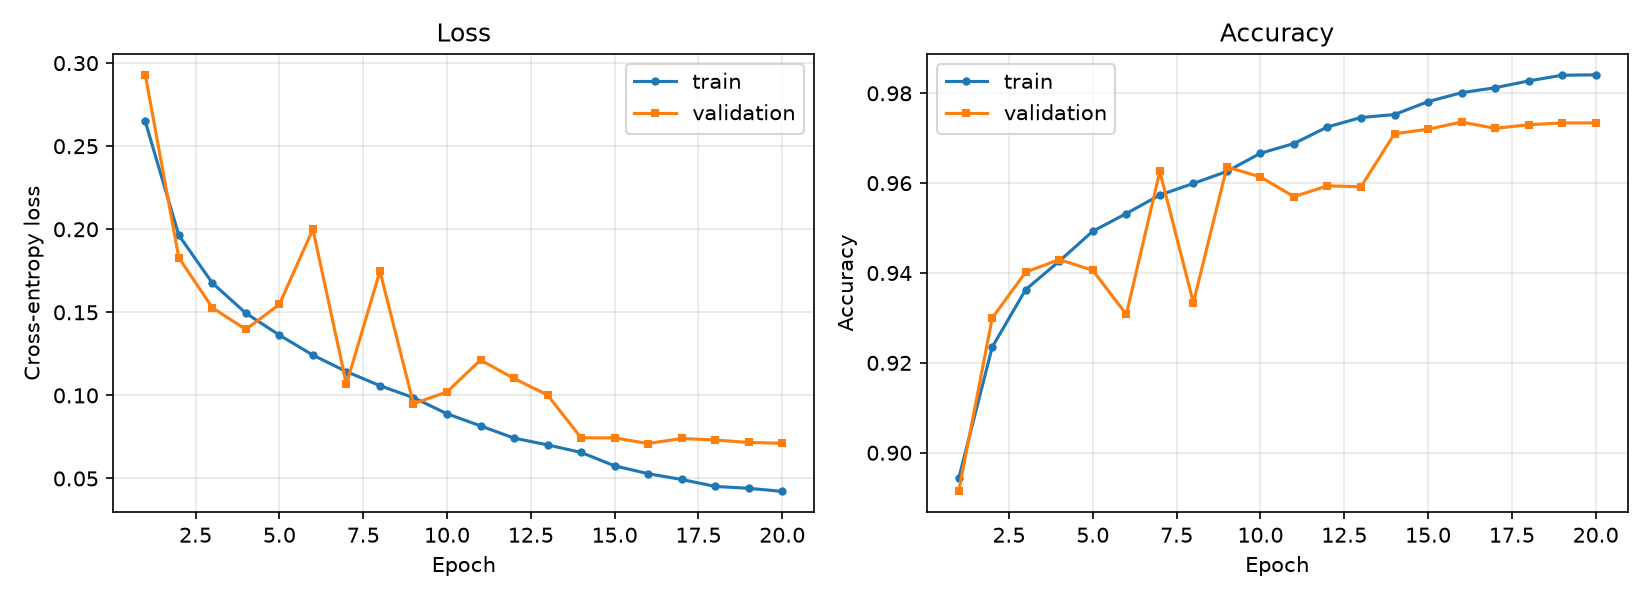
\includegraphics[width=0.95\textwidth]{../reports/figures/training_curves.png}
\caption{Trening i validacioni gubitak (levo) i ta\v cnost (desno) u
zavisnosti od epohe.}
\label{fig:curves}
\end{figure}

\subsection{Kvantitativno pore\dj enje}
Tabela~\ref{tab:comparison} upore\dj uje KNM sa dve samostalno razvijene
referentne metode na test skupu od $10{,}000$ slika, koriste\'ci ta\v cnost,
preciznost, odziv, $F_1$ meru i ROC-AUC. KNM nadma\v suje obe referentne metode
po svakoj meri sa velikom razlikom. Konkretno, zamena linearnog modela
logisti\v cke regresije nelinearnim MLP pobolj\v sava ta\v cnost sa $81.6\%$ na
$88.0\%$, ali dodavanje konvolucione strukture (deljenje te\v zina i prostorna
lokalnost) donosi mnogo ve\'ci skok na $97.3\%$. Ovo je u skladu sa
literaturom~\cite{krizhevsky2012imagenet,simonyan2015very} i potvr\dj uje da je
prostorno izdvajanje obele\v zja presudni \v cinilac za ovaj zadatak.

\begin{table}[h]
\centering
\caption{Performanse na test skupu za zadatak binarne detekcije vozila.
Najbolja vrednost po koloni je \textbf{podebljana}.}
\label{tab:comparison}
\begin{tabular}{lccccc}
\toprule
\textbf{Model} & \textbf{Ta\v cnost} & \textbf{Preciznost} & \textbf{Odziv} & \textbf{$F_1$} & \textbf{ROC-AUC} \\
\midrule
Logisti\v cka regresija    & 0.8156 & 0.7906 & 0.7333 & 0.7608 & 0.8790 \\
MLP (bez konvolucija)     & 0.8804 & 0.8542 & 0.8453 & 0.8497 & 0.9434 \\
\textbf{VehicleCNN (na\v se)} & \textbf{0.9727} & \textbf{0.9686} & \textbf{0.9630} & \textbf{0.9658} & \textbf{0.9965} \\
\bottomrule
\end{tabular}
\end{table}

\subsection{Analiza gre\v saka}
Slika~\ref{fig:cm} prikazuje matricu konfuzije KNM na test skupu. Gre\v ske su
pribli\v zno uravnote\v zene izme\dj u dva tipa: propu\v stena vozila naspram
slika koje nisu vozila a ozna\v cene su kao vozila. Preciznost ($0.969$) i odziv
($0.963$) su bliski, \v sto ukazuje na to da nema jake pristrasnosti ka bilo
kojoj klasi uprkos neravnote\v zi klasa $40/60$. Slike~\ref{fig:roc}
i~\ref{fig:pr} prikazuju ROC krivu i krivu preciznost--odziv; ROC-AUC od
$0.9965$ pokazuje da je klasifikator odli\v can u rangiranju i da se prag
odlu\v civanja mo\v ze slobodno pode\v savati za primene koje favorizuju ve\'ci
odziv ili ve\'cu preciznost.

\begin{figure}[h]
\centering
\begin{subfigure}{0.32\textwidth}
  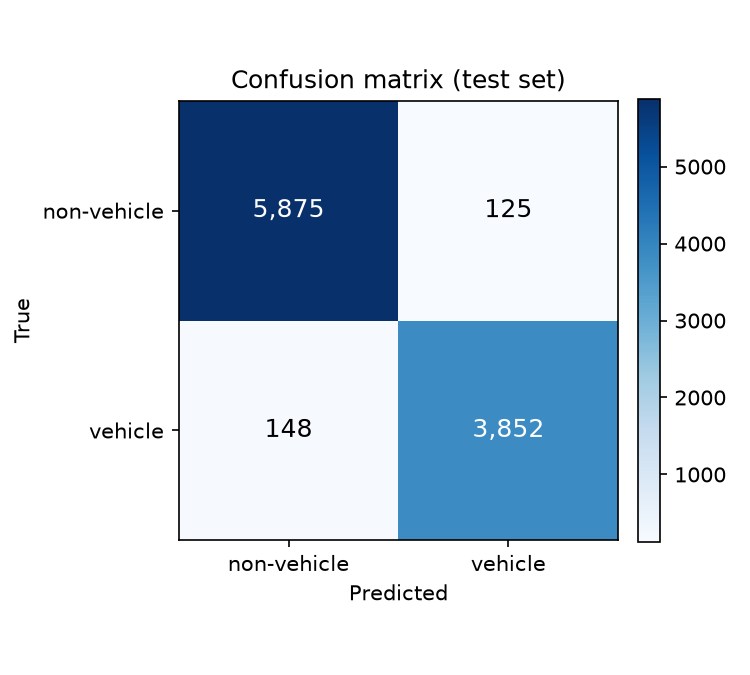
\includegraphics[width=\textwidth]{../reports/figures/confusion_matrix.png}
  \caption{Matrica konfuzije}
  \label{fig:cm}
\end{subfigure}\hfill
\begin{subfigure}{0.32\textwidth}
  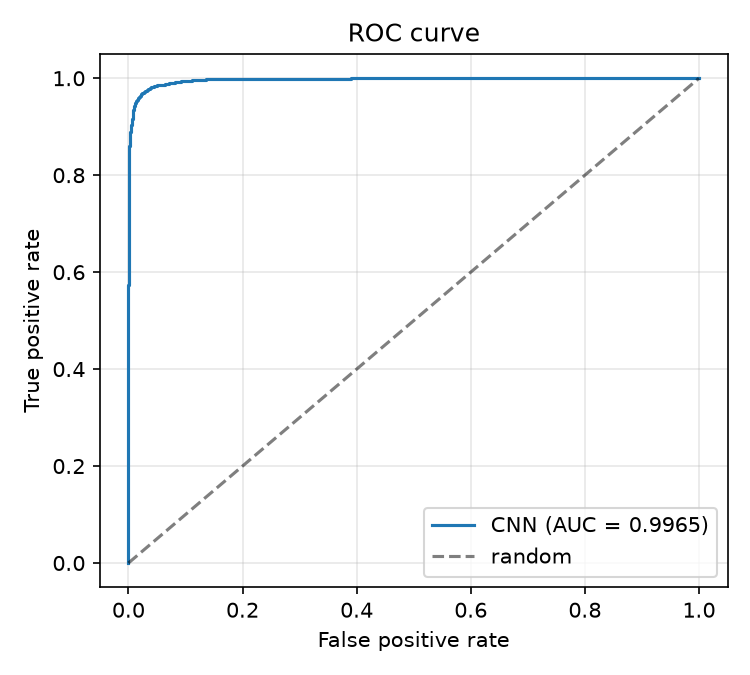
\includegraphics[width=\textwidth]{../reports/figures/roc_curve.png}
  \caption{ROC kriva}
  \label{fig:roc}
\end{subfigure}\hfill
\begin{subfigure}{0.32\textwidth}
  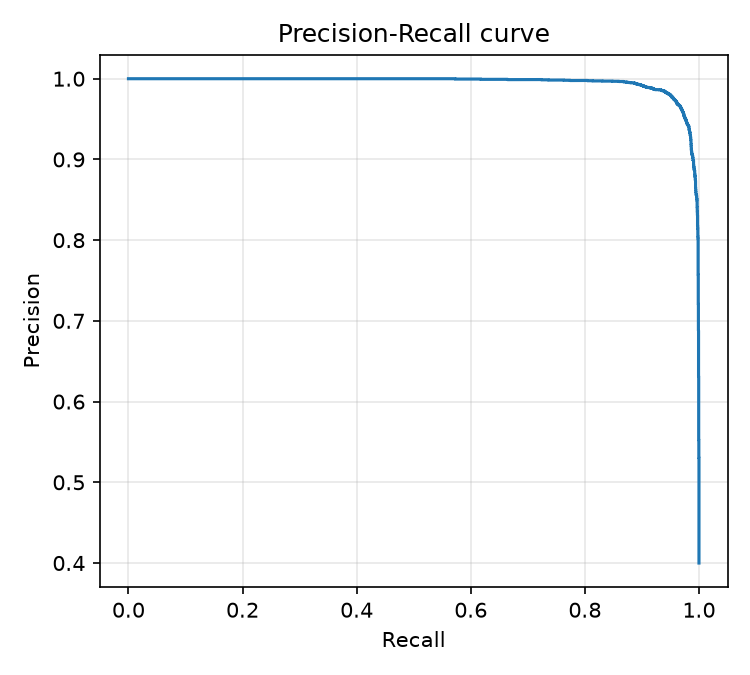
\includegraphics[width=\textwidth]{../reports/figures/pr_curve.png}
  \caption{Kriva preciznost--odziv}
  \label{fig:pr}
\end{subfigure}
\caption{Dijagnosti\v cki grafici za KNM na test skupu.}
\label{fig:diagnostics}
\end{figure}

\subsection{Kvalitativni rezultati na jednostavnim primerima}
Kao \v sto je zahtevano, demonstriramo metodu na jednostavnim, pojedina\v cno
vizuelizovanim test slikama. Slika~\ref{fig:samples} prikazuje dvanaest
nasumi\v cno izabranih test slika zajedno sa ta\v cnom oznakom, predvi\dj enom
oznakom i predvi\dj enom verovatno\'com $P(\text{vozilo})$. Model klasifikuje
jasne primere (automobili, brodovi, kamioni, \v zivotinje) sa gotovo izvesnom
pouzdano\v s\'cu, dok te\v zi ili netipi\v cni prikazi (npr.\ avion vi\dj en iz
neobi\v cnog ugla) dobijaju predvi\dj anja ni\v ze pouzdanosti ali i dalje
ta\v cna, \v sto je \v zeljeno pona\v sanje.

\begin{figure}[h]
\centering
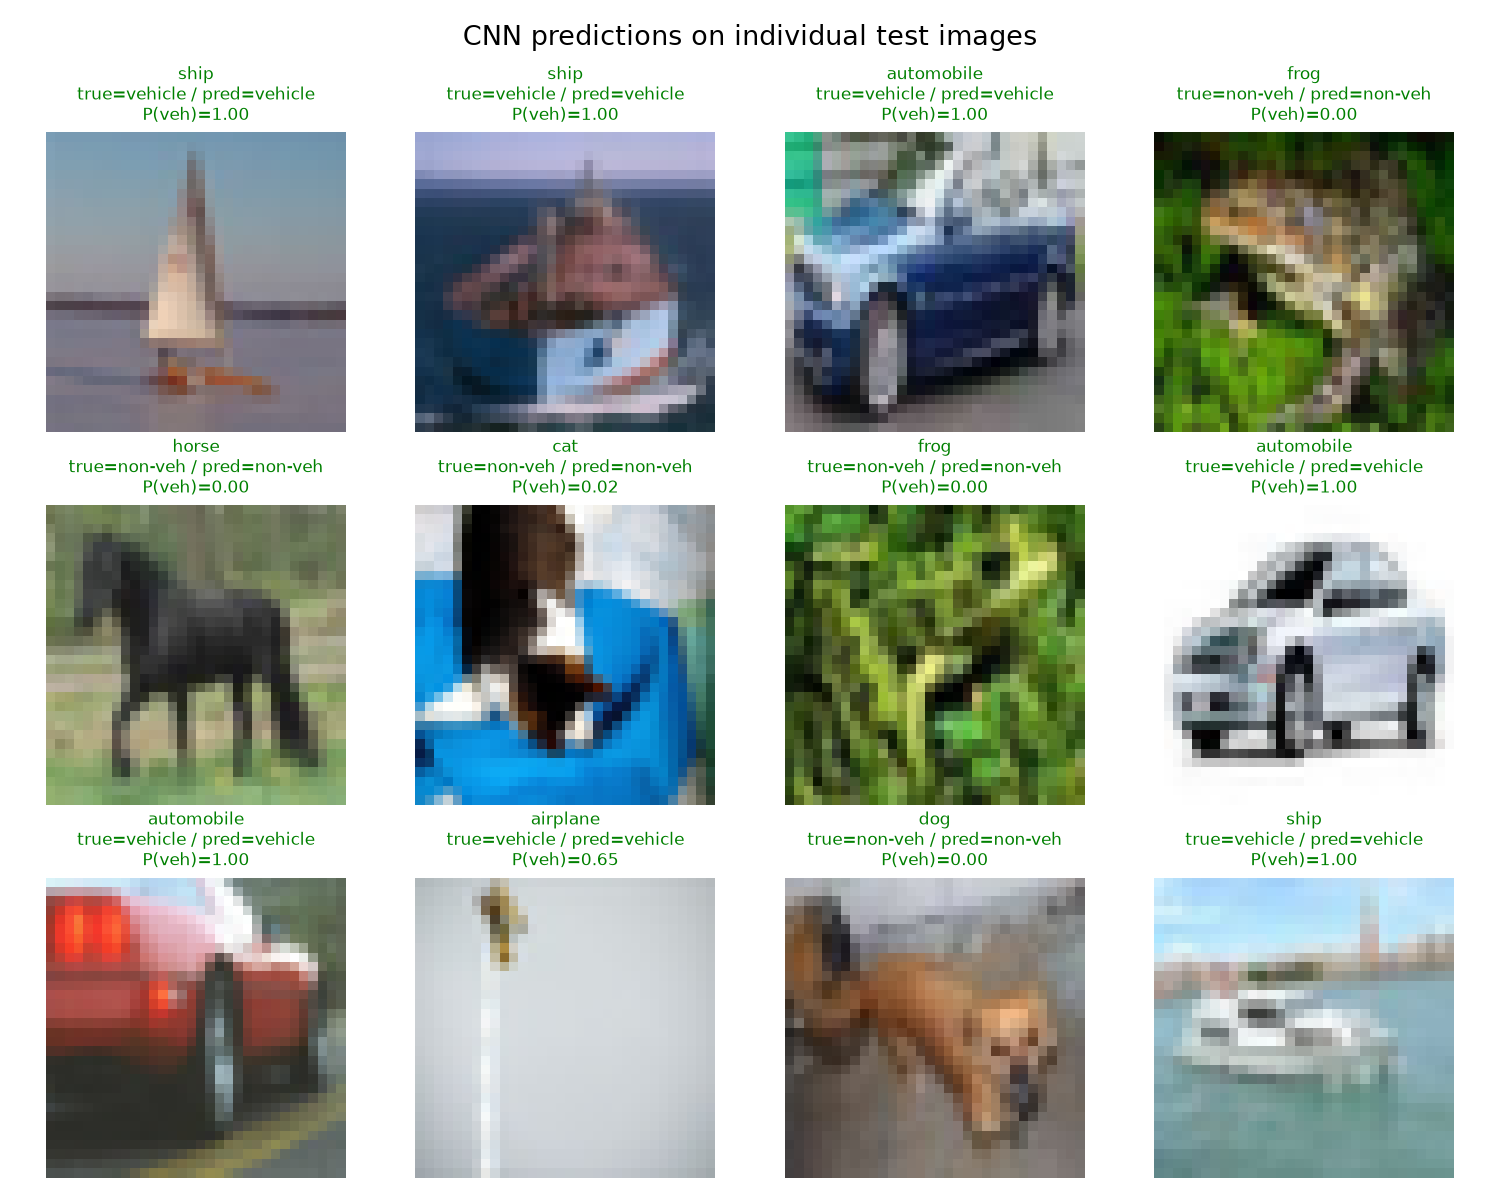
\includegraphics[width=0.9\textwidth]{../reports/figures/sample_predictions.png}
\caption{Predvi\dj anja KNM na pojedina\v cnim test slikama. Naslovi prikazuju
originalnu klasu CIFAR-10, binarne ta\v cne/predvi\dj ene oznake i
$P(\text{vozilo})$; zeleni naslovi ozna\v cavaju ta\v cna predvi\dj anja.}
\label{fig:samples}
\end{figure}

% ===========================================================================
\section{Zaklju\v cak}
% ===========================================================================
Reprodukovali smo standardnu metodologiju konvolucionih neuronskih mre\v za za
klasifikaciju slika i primenili je na binarnu detekciju vozila na skupu
podataka CIFAR-10. Na\v sa kompaktna mre\v za u stilu VGG dostigla je ta\v cnost
od $97.27\%$ na test skupu i ROC-AUC od $0.9965$, jasno nadma\v suju\'ci
referentne metode logisti\v cke regresije ($81.6\%$) i potpuno povezanog MLP
($88.0\%$) koje smo razvili radi pore\dj enja. Kontrolisano pore\dj enje izoluje
doprinos konvolucione arhitekture: najve\'ci deo pobolj\v sanja u odnosu na
nelinearni MLP poti\v ce upravo od deljenja te\v zina i prostorne lokalnosti,
\v sto je u skladu sa objavljenom literaturom.

Nagla\v savamo da je ovaj rad verna reprodukcija postoje\'cih ideja
\cite{lecun1998gradient,krizhevsky2012imagenet,simonyan2015very}, a ne nova
metoda, i ne tvrdimo da nadma\v sujemo najsavremenija re\v senja; specijalizovane
arhitekture poput ResNet~\cite{he2016deep} posti\v zu vi\v su ta\v cnost na
punom skupu CIFAR-10. Ostaje nekoliko ograni\v cenja i pravaca za dalji rad:
\begin{itemize}
  \item \textbf{Detekcija, ne samo klasifikacija.} Trenutni model odlu\v cuje
        samo \emph{da li} je vozilo prisutno. Pro\v sirenje na lokalizaciju
        vozila grani\v cnim okvirima, npr.\ integracijom osnove u detektor
        Faster R-CNN~\cite{ren2015faster} ili YOLO~\cite{redmon2016you}, jeste
        prirodan slede\'ci korak.
  \item \textbf{Podaci vi\v se rezolucije i iz stvarnog sveta.} Slike skupa
        CIFAR-10 su samo $32\times 32$. Evaluacija na slikama saobra\'caja vi\v se
        rezolucije bolje bi odra\v zavala uslove primene.
  \item \textbf{Sna\v znije arhitekture i regularizacija.} Rezidualne
        veze~\cite{he2016deep}, dublje mre\v ze i savremene strategije
        augmentacije verovatno bi smanjile deo preostale gre\v ske.
  \item \textbf{Finije kategorije vozila.} Razlikovanje \emph{tipova} vozila
        (automobil naspram kamiona naspram broda) umesto jedne binarne oznake
        jeste korisno pro\v sirenje.
\end{itemize}
U celini, eksperimenti potvr\dj uju da je \v cak i mala KNM sna\v zno i
prakti\v cno re\v senje za detekciju prisustva vozila.

% ===========================================================================
\section*{Reproducibilnost i tu\dj i kod}
% ===========================================================================
\addcontentsline{toc}{section}{Reproducibilnost i tu\dj i kod}
Sav kod je originalan i napisan od strane autora, uz izuzetak op\v stepoznatih
API-ja biblioteka (PyTorch~\cite{paszke2019pytorch}, torchvision,
scikit-learn~\cite{pedregosa2011scikit}, Matplotlib, NumPy) kori\v s\'cenih na
standardan, dokumentovan na\v cin. Skup podataka
CIFAR-10~\cite{krizhevsky2009learning} preuzima se automatski putem
torchvision-a sa zvani\v cnog izvora. Konstante normalizacije skupa CIFAR-10 kao
i dizajn u stilu VGG i recept za treniranje (augmentacija podataka, BatchNorm,
dropout, AdamW, kosinusni raspore\dj iva\v c) prate uobi\v cajenu praksu
utemeljenu u citiranoj literaturi. Kompletan kod, ovaj dokument i sve slike
dostupni su u javnom GitHub repozitorijumu, \v sto omogu\'cava potpunu
reprodukciju prikazanih rezultata.

% ===========================================================================
\bibliographystyle{ieeetr}
\bibliography{references}
% ===========================================================================

\end{document}

